\part{最优化理论}
\section{预备知识}
\subsection{概念与形式化}

\newcommand{\SubjectTo}{\mathrm{s.t.}}

\begin{definition}[极值问题及不同约束及记号]
    形如
    \[
        \min f(\VectorComma{x}{n})
    \]
    的问题称为\textkw{无约束问题}。
    形如
    \[
        \begin{array}{ll}
            \min & f(\VectorComma{x}{n}) \\
            \SubjectTo & h_i(\VectorComma{x}{n})=0,i=1,2,\dots,l \\
            & s_j(\VectorComma{x}{n})\geq 0,j=1,2,\dots,m \\
        \end{array}
    \]
    或记作
    \[
        \begin{array}{ll}
            \min & f(\vec{x}) \\
            \SubjectTo & \vec{h}(\vec{x})=\vec{0}\\
            & \vec{s}(\vec{x})\geq \vec{0}
        \end{array}
    \]
    的问题是\textkw{有约束问题}。
    其中$f(\vec{x})$为\textkw{目标函数},
    $\vec{h}(\vec{x})=\vec{0}$为\textkw{等式约束},
    $\vec{s}(\vec{x})\geq\vec{0}$为\textkw{不等式约束}。
\end{definition}

对于$\max g(\VectorComma{x}{n})$,通常转化为$\min f(\VectorComma{x}{n}),f=-g$处理;
对于$s(x)\leq 0$的约束也按$-s(x)\geq 0$处理。

\begin{definition}[容许集~容许解]
    满足约束的$\vec{x}$的范围记为$D$,称为\textkw{容许集/可行集},
    其中的$\vec{x}$的取值称为\textkw{容许解/可行解}。
\end{definition}

\begin{definition}[极小点及其分类]
    对$\vec{x}^*\in D$,若$\forall \vec{x}\in D, f(\vec{x}^*)\leq f(\vec{x})$,
    则$\vec{x}^*$称为\textkw{最优点/极小点},$f(\vec{x}^*)$称为\textkw{最优值/极小值},
    $(\vec{x}^*,f(\vec{x}^*))$称为\textkw{最优解}。
    根据局部或全局分为\textkw{局部极小点}和\textkw{全局极小点}。
    在这个范围内,取值达到最小,称为\textkw{严格极小点},取值没有比它更小的,称为\textkw{非严格极小点}。
\end{definition}

\subsection{简单的情况}

\begin{itemize}
    \item 令一阶导数或梯度为$0$
    \item Lagrange乘子法
    \item 图解法
\end{itemize}

\subsection{梯度与Hesse矩阵}
\subsubsection{梯度}

\begin{definition}[可微]
    对$f:\mathbb{R}^n\to\mathbb{R},x_0\in D$,若$\exists l\in\mathbb{R}^n,\forall p\in\mathbb{R}^n,$有:
    \[
        \lim _{\| \vec{p} \| \rightarrow 0} \frac{f(\vec{x}_{0}+\vec{p})-f(\vec{x}_{0})-\vec{l}^{T} \vec{p}}{\|\vec{p}\|}=0
    \]
    则称$f$在$x_0$处可微。
    此时一阶导数总存在,且为$\vec{l}$的各个分量:
    \[
        \nabla f = \left( \frac{\partial f}{\partial x_1}, \frac{\partial f}{\partial x_2}, \dots, \frac{\partial f}{\partial x_n} \right)\Transpose
    \]
    定义为在$\vec{x}$处的梯度。
\end{definition}

\begin{property}
    对多元函数的梯度,以下性质成立:
    \begin{itemize}
        \item 梯度处处垂直于等值面。
        \item 梯度是$x_0$处变化最快方向。
        \item 对$\exists \delta>0,\forall t\in (0,\delta), f(\vec{x}_0+t\vec{p})>f(\vec{x}_0)$则称为上升方向,否则为下降方向。
    \end{itemize}
\end{property}

方向导数的定义略。
上升方向、下降方向取决于方向导数的正负。
方向导数大小为梯度与方向向量的内积。

标量值函数对向量求梯度的常见公式:
\begin{gather*}
    \nabla C = 0 \\
    \nabla (\vec{b}\Transpose \vec{x})=\vec{b} \\
    \nabla (\vec{x}\Transpose Q \vec{x})=2Q\vec{x} \\
\end{gather*}

\subsubsection{向量值函数梯度}

\begin{definition}[向量值函数可微]
    \[
        \lim _{\| \vec{p} \| \rightarrow 0} \frac{\vec{g}\left(\vec{x}_{0}+\vec{p}\right)-\vec{g}\left(\vec{x}_{0}\right)-\nabla \vec{g}\left(\vec{x}_{0}\right)^{T} \vec{p}}{\|\vec{p}\|}=\overrightarrow{0}
    \]
    称为向量值函数$\vec{g}$在$\vec{x}_0$处可微,其中
    \[
        \nabla \vec{g}(\vec{x}_0) = \left( \frac{\partial g_j(\vec{x}_0)}{\partial x_i} \right)_{n\times m}
    \]
    称为向量值函数在$\vec{x}_0$处的梯度。
    $\nabla\vec{g}\Transpose$称为Jacobi矩阵。
\end{definition}

向量值函数求梯度的常见公式:
\begin{gather*}
    \nabla \vec{c} = \bm{0} \\
    \nabla \vec{x} = I \\
    \nabla (A\vec{x}) = A\Transpose \\
\end{gather*}

\begin{definition}
    记$\nabla^2 f(x) = \nabla[\nabla f(x)] = \left( \frac{\partial^2 f}{\partial x_i \partial x_j} \right)_{n\times n}$
    为$f(\vec{x})$的二阶导数,也称为$f(\vec{x})$的\textkw{Hesse矩阵}。
\end{definition}

\begin{theorem}
    对$\varphi(t) = f(\vec{x}+t\vec{p})$,有$\varphi'(t)=\nabla f(\vec{x}+t\vec{p})\Transpose \vec{p}$,
    $\varphi''(t)=\vec{p}\Transpose \nabla f(\vec{x}+t\vec{p}) \vec{p}$,因此可得三项泰勒展开式:
    \[
        f(\vec{x}+\vec{p})=f(\vec{x})+\nabla f(\vec{x})^{T} \vec{p}+\frac{1}{2} \vec{p}^{T} \nabla^{2} f(\vec{x}) \vec{p}+o(\|\vec{p}\|)
    \]
\end{theorem}

\subsection{凸函数与凸规划}
\subsubsection{凸集}

\begin{definition}[凸组合~严格凸组合]
    $x=\sum_i a_i x_i$,其中$\sum_i a_i=1$。若$a_i\geq 0$,称为凸组合,若$a_i>0$,称为严格凸组合。
\end{definition}

\begin{definition}[凸集]
    集合中任意两点的任意凸组合属于集合,称为凸集。
\end{definition}

\begin{theorem}[凸集判定]
    凸集,当且仅当,集合中任意两点的中点总是在集合内。
\end{theorem}

超平面、椭球等都是凸集,平面、半平面也是。特别规定空集也是。

\begin{theorem}
    凸集的交集是凸集。
\end{theorem}

\subsubsection{凸函数}

\begin{definition}
    设$C$为凸集,对$f:C\subseteq\mathbb{R}^n\to \mathbb{R}$,
    对任意互异两点$\vec{x}_1,\vec{x}_2$,对任意和为$1$且非负的$\alpha_1,\alpha_2$,
    总有$f(\alpha_1\vec{x}_1+\alpha_2\vec{x}_2)\leq \alpha_1 f(\vec{x}_1)+\alpha_2 f(\vec{x}_2)$,
    则称$f$为定义在凸集$C$上的\textkw{凸函数}。
    若对任意和为$1$且正的$\alpha_1,\alpha_2$有上式且取不到等号,则称$f$为\textkw{严格凸函数}。
    对凸集$C$上的函数$g$,若$f=-g$为凸函数,称$g$为\textkw{凹函数}。
\end{definition}

\begin{theorem}
    有限个凸函数的非负组合仍然是凸函数。
\end{theorem}

\begin{theorem}
    对凸集$C$上的凸函数$f$,水平集$\{\vec{x}\mid f(\vec{x})\leq \beta, \vec{x}\in C\}$是凸集。
\end{theorem}

\begin{theorem}[凸函数判定]
    设$C$为凸集,$f:C\subseteq\mathbb{R}^n\to\mathbb{R}$为可微函数,则:
    \begin{itemize}
        \item $f$为凸函数$\Leftrightarrow \forall\vec{x}_1,\vec{x}_2,f(\vec{x}_2)>f(\vec{x}_1) + \nabla f(\vec{x}_1)\Transpose (\vec{x}_2-\vec{x}_1)$
        \item $f$为严格凸函数$\Leftrightarrow \forall\vec{x}_1\neq\vec{x}_2,f(\vec{x}_2)>f(\vec{x}_1) + \nabla f(\vec{x}_1)\Transpose (\vec{x}_2-\vec{x}_1)$
    \end{itemize}
\end{theorem}

\begin{theorem}
    $C$非空开凸集,$f$二阶可微,则$f$为凸函数$\Leftrightarrow \nabla^2 f$在$C$上半正定。
\end{theorem}

\begin{theorem}
    $C$非空凸集,$f$二阶可微,则$f$为严格凸函数$\Rightarrow \nabla^2 f$在$C$上正定。
\end{theorem}

\subsubsection{凸规划}

\begin{definition}[凸规划]
    设$C$是凸集,$f$是凸集上的凸函数。则问题$\min f(\vec{x}) \SubjectTo \vec{x}\in C$称为\textkw{凸规划问题}。
\end{definition}

对有约束情况,若等式约束$\vec{h}(\vec{x})=0$是线性函数,$s_i(\vec{x})$都是凹函数,则容许集是凸集,
在容许集上的凸函数也是一种凸规划问题。

\begin{property}
    凸规划具有以下性质:
    \begin{itemize}
        \item 极小点$\vec{x}^*$是全局极小点。
        \item 严格凸函数的极小点是唯一全局极小点。
        \item 极小点集合是凸集。
    \end{itemize}
\end{property}

\begin{theorem}
    $C$非空凸集,$f$是$C$上可微凸函数,则:
    \[
        \vec{x}^*\text{是极小点} \Leftrightarrow \forall\vec{x}\in C, \nabla f(\vec{x}^{*})\Transpose(\vec{x}-\vec{x}^*)
    \]
    ,即极小点的任意方向都不是下降方向。
\end{theorem}

\begin{corollary}
    $C$非空凸集,$f$是$C$上可微凸函数,则:
    \[
        \nabla f(\vec{x}^*)=\vec{0} \Rightarrow \vec{x}^*\text{是极小点}
    \]
\end{corollary}

\subsubsection{二次规划}
\begin{definition}[二次函数~正定二次函数]
    多元二次函数表示为$f(\vec{x}) = \frac{1}{2}\vec{x}\Transpose Q\vec{x} + \vec{b}\Transpose\vec{x} + c$,
    若$Q>0$,称为正定二次函数。
\end{definition}

对二次函数$f$,有$\nabla f(\vec{x})=Q\vec{x}+\vec{b}$,$\nabla^2 f(\vec{x}) = Q$。
因此有:
\begin{itemize}
    \item $Q$正定的二次函数是严格凸函数。
    \item $Q$半正定的二次函数的凸函数。
\end{itemize}

\begin{definition}[二次规划]
    最优化问题
    $\min f(\vec{x})=\frac{1}{2}\vec{x}\Transpose Q\vec{x} + \vec{b}\Transpose\vec{x} + c ~\linebreak[1] \SubjectTo A\vec{x}\geq \vec{p}, C\vec{x} = \vec{d}$
    称为二次规划问题,简称二次规划。
    若$Q$半正定(或正定),称为二次凸规划问题。
\end{definition}

\subsection{极小点判定}

\begin{theorem}
    $f$是$D$上的函数,有连续一阶偏导,$\vec{x}^*\in \operatorname{int}D$,则
    $\vec{x}^*\text{是局部极小点} \Rightarrow \nabla f(\vec{x}^*)=\vec{0}$
\end{theorem}

\begin{theorem}
    $C$非空开凸集,$f$是$C$上可微凸函数,$\vec{x}^*\in C$,则
    $\vec{x}^*\text{是全局极小点} \Leftrightarrow \nabla f(\vec{x}^*)=\vec{0}$
\end{theorem}

\begin{definition}[驻点]
    $f$是$D$上的可微函数,$\vec{x}^*\in D$,若
    $\nabla f(\vec{x}^*)=\vec{0}$,则称$\vec{x}^*$为$f(\vec{x})$的\textkw{驻点}。
\end{definition}

\begin{theorem}
    $f$是$D$上函数,有连续二阶偏导,$\vec{x}^*\in D$,则
    $\nabla f(\vec{x}^*)=\vec{0}, \nabla^2 f(\vec{x}^*)>0 \Rightarrow\vec{x}^*\text{是严格局部极小点}$
\end{theorem}

\begin{theorem}
    $f$是$\mathbb{R}^n$上函数,有连续二阶偏导,$\vec{x}^*\in \mathbb{R}^n$,则
    $\nabla f(\vec{x}^*)=\vec{0}, \forall \vec{x}\in N(\vec{x}^*,\delta), \nabla^2 f(\vec{x})\geq 0 \Rightarrow\vec{x}^*\text{是局部极小点}$
\end{theorem}

因此正定二次函数有唯一极小点$\vec{x}^*=-Q^{-1}\vec{b}$。

若极小点附近Hesse矩阵正定,等值面近似同心椭球面族。

\subsection{下降迭代算法}
\subsubsection{下降迭代算法}

\begin{definition}
    在集合$X$上选取一个初始值$x_0$,然后依据某种规则$A$从第$k$次迭代点$x_k$得到第$k+1$次迭代点$x_{k+1}$。
    则称为迭代算法。
    对最优化问题,$X$为容许集时,若迭代过程中使得$f(x_{k+1})<f(x_k)$,则称为下降迭代算法。
\end{definition}

算法中的迭代步骤:
\begin{enumerate}
    \item 选定初始点$\vec{x}_0$,设置$k=0$
    \item 确定迭代方向$\vec{p}_k$
    \item 确定迭代步长$t_k$
    \item 迭代$\vec{x}_{k+1}=\vec{x}_k+t_k \vec{p}_k$
    \item 判定是否符合终值准则。若未结束,返回第2步。
\end{enumerate}

\subsubsection{直线搜索}
已确定$\vec{p}_k$后选择$t_k$。
\begin{definition}
    选择步长$t_k$时选择使得
    $\min\limits_t f(\vec{x}_k+t\vec{p}_k)$的$t$作为$t_k$,
    这个方法称为直线搜索。其中取值$t_k$称为最优步长因子。
\end{definition}

优点是下降量最多,但同时有计算量大的缺点。

\begin{property}
    对直线搜索的结果$\vec{z}=\vec{x}_k+t_k\vec{p}_k$有$\nabla f(\vec{z})\Transpose \cdot \vec{p}_k=0$
\end{property}

\subsubsection{计算终止准则}
理想:$\|\vec{x}^*-\vec{x}\|<\varepsilon$。但$\vec{x}^*$未知因此需要使用其他方法逼近。

简单用变化量刻画终止准则:
\[
    \begin{cases}
        \| \vec{x}_{k+1} - \vec{x}_k \| < \varepsilon_1\\
        \| f(\vec{x}_{k+1}) - f(\vec{x}_k) \| < \varepsilon_2
    \end{cases}
\]

无量纲处理:
\[
    \begin{cases}
        \frac{\| \vec{x}_{k+1} - \vec{x}_k \|}{\|\vec{x}_k\|+1} < \varepsilon_1\\
        \frac{\| f(\vec{x}_{k+1}) - f(\vec{x}_k) \|}{\|f(\vec{x}_k)\|+1} < \varepsilon_2
    \end{cases}
\]

也可以结合$\|\nabla f\|<\varepsilon_3$进行判断。

\section{线性规划*}

\begin{definition}
    目标函数和等式约束都是线性,且不等式约束各$x$非负的问题,
    $\min \sum c_i x_i \SubjectTo \sum a_{ij} x_j = b_i, x_i\geq 0$,称为线性规划问题。
    一般也记作$\min C\vec{x} \SubjectTo A\vec{x}=\vec{b}$。
\end{definition}

线性规划的最优解总是出现在顶点。

\section{无约束优化方法}

无约束优化问题分为根据梯度或Hesse矩阵的方法和直接方法。
前一类因为需要计算梯度和Hesse矩阵,对函数有一定要求,后一类适应性强但收敛较慢。
前者按梯度进行搜索,首先我们需要再次考虑直线搜索问题。
也就是求解一元函数极小化问题$\min \varphi(t)$的方法。

\subsection{直线搜索}

对$\varphi'(t)=0$可求解的问题,显然二分法查找零点是最朴素的方法。
此外的分为精确的和不精确的两类。
精确的直线搜索方法包括下面的区间收缩和函数逼近两种。

\subsubsection{区间收缩法}

\begin{definition}[单谷函数]
    对函数$\varphi(t)$,存在全局极小点$t^*$,对任意$t_1<t_2$,有:
    若$t_1<t_2\leq t^*$,则$f(t_1)>f(t_2)$;若$t^*\leq t_1<t_2$,则$f(t_1)<f(t_2)$。
    即$\varphi(t)$在定义域上,$t^*$的左侧严格单调递减,右侧严格单调递增。
    称这样的$\varphi(t)$为单谷函数。
\end{definition}

\begin{definition}[搜索区间]
    对函数$\varphi(t)$,记其全局极小点为$t^*$,
    对区间$[t_1,t_2]$,若$t^*\in [t_1,t_2]$,则称为$\varphi(t)$极小点的一个搜索区间,
    通常记作$\{t_1,t_2\}$。有时也选择一个$t_3\in (t_1,t_2)$记作$\{t_1,t_3,t_2\}$。
\end{definition}
单谷函数的定义域就是一个搜索区间。

\begin{theorem}
    对单谷函数$\varphi(t)$极小点的一个搜索区间$\{a,b\}$,
    任取$t_1,t_2\in (a,b) t_1<t_2$,则:
    若$\varphi(t_1)\leq \varphi(t_2)$,则$\{a,t_2\}$是一个搜索区间;
    若$\varphi(t_1)\geq \varphi(t_2)$,则$\{t_1,b\}$是一个搜索区间。
\end{theorem}

因此,得到确定搜索区间的算法。
\begin{enumerate} % 不确定正确性
    \item 确定初始点$t_0$与步长$h$
    \item 计算$\varphi_0=\varphi(t_0),t_2=t_0+h,\varphi_2=\varphi(t_2)$
    \item 若$\varphi_0 \leq \varphi_2$,令$t_1=t_0,\varphi_1=\varphi_0,h=-h$)(翻转搜索方向),转5;否则转4
    \item 令$t_1=t_0,\varphi_1=\varphi_0,t_0=t_2,\varphi_0=\varphi_2,h=2h$(前进并倍增区间长度)
    \item $t_2=t_0+h,\varphi_2=\varphi(t_2)$。若$\varphi_2>\varphi_0$转6;否则转4(前进,若完成则结束,否则倍增)
    \item 令$a=\min\{t_1,t_2\},b=\max\{t_1,t_2\}$,得到搜索区间$\{a,b\}$
\end{enumerate}
得到$t_0<t_1<t_2$且公差为$h$,且$\varphi_0>\varphi_1<\varphi_2$的搜索区间。
$t_0$与$h$需要事先指定,
经验上,初始步长$h$选择$1$,然后在第$k$次更新中,选择$h=\beta\frac{\|\vec{x}_k - \vec{x}_{k-1}\|}{\|\vec{p}_k\|}$。

\paragraph{黄金分割法}
若考虑复用上次的函数值,使用其中仍然处在中间的点,
则问题转化为保证子区间$\{a,t_1,t_2\}$或$\{t_1,t_2,b\}$中间的点仍然处在类似比例的位置,
然后就会得到黄金分割比。

对$a,b$取$\beta=\frac{\sqrt{5} - 1}{2}$,然后$t_2=\beta (b-a)+a, t_1=a+b-t_2$,
则判断保留$\{t_1,t_2,b\}$时,$t_2$在区间的比例成为新的$t_1$,
保留$\{a,t_1,t_2\}$时,$t_1$在区间中的比例成为新的$t_2$。

区间每次缩小到原来的$\beta$倍,较二分法求$\varphi'(t)=0$缩小速度慢,但是求值的时间会更快。

\subsubsection{函数逼近法——二次插值法}
二次插值法,也称抛物线插值法,是一种函数逼近法。适用于连续单谷函数求极小值。

算法:
\begin{enumerate}
    \item 给定搜索区间$\{t_1,t_2,t_3\}$,过$(t_1,\varphi_1),(t_2,\varphi_2),(t_3,\varphi_3)$
        拟合抛物线$Q(t)=pt^2+qt+r$,则得到极小值点$t_4=-\frac{q}{2p}$。
    \item 检查终止条件$\frac{|\varphi_4-\varphi_2|}{|\varphi_2|+1} < \epsilon$。
    \item 比较$t_4,t_2$以及$\varphi_4,\varphi_2$。
    \item 以比较结果选择新的搜索区间。
        若$t_1<t_2<t_4<t_3$:若$\varphi_2<\varphi_4$,取左侧$\{t_1,t_2,t_4\}$;
        若$\varphi_2<\varphi_4$,取右侧$\{t_2,t_4,t_3\}$。
        若$t_1<t_4<t_2<t_3$:若$\varphi_4>\varphi_2$,取右侧$\{t_4,t_2,t_3\}$;
        若$\varphi_4<\varphi_2$,取左侧$\{t_1,t_4,t_2\}$。
    \item 迭代。
\end{enumerate}

\subsubsection{不精确一维搜索}
Goldstein和Powell指出了关于设计不精确一维搜索的迭代方法的两个条件。
\begin{gather*}
    f\left(\vec{x}_{k}\right)-f\left(\vec{x}_{k+1}\right) \geq-\rho t_{k} \nabla f\left(\vec{x}_{k}\right)^{T} \vec{p}_{k}\\
    \nabla f\left(\vec{x}_{k+1}\right)^{T} \vec{p}_{k} \geq \sigma \nabla f\left(\vec{x}_{k}\right)^{T} \vec{p}_{k}
\end{gather*}
其中$\rho,\sigma$为满足$0<\rho<\sigma<1$的常数。

\subsection{最速下降法}
回顾前面梯度部分的定义,最速下降方向指梯度的反方向。
方便起见,记$f_k=f(\vec{x}_k),\vec{g}_k=\nabla f(\vec{x}_k)$。

基本思想:
第$k$次迭代时,当前已迭代得到$\VectorComma{\vec{x}}{k}$,
取搜索方向$\vec{p}_k=-\nabla \vec{x}_k$,
然后选择使得$\min\limits_t f(\vec{x}_k + t \vec{p}_k)$的步长$t_k$进行迭代。

\begin{property}
    每次迭代有$\nabla f(\vec{x}_k)\perp \nabla f(\vec{x}_{k+1})$,即
    \[
        \vec{g}_k\Transpose\vec{g}_{k+1} = 0
    \]
\end{property}

以正定二次函数为例,$\vec{g}_k=Q\vec{x}_k+\vec{b}$,代入$\vec{x}_{k+1}=\vec{x}_k-t_k\vec{g}_k$,
因此有$\vec{g}_{k+1} = Q\vec{x}_{k+1}+\vec{b} = Q\vec{x}_k - t_k Q \vec{g}_k = \vec{g}_k - t_k Q \vec{g}_k$,
从$\vec{g_k}\Transpose (\vec{g}_k - t_k Q \vec{g}_k) = 0$,
可解出对正定二次函数:
\[
    t_k=\frac{\vec{g}_k\Transpose\vec{g}_k}{\vec{g}_k\Transpose Q \vec{g}_k}
\]

\begin{property}[收敛性]
    对任意点收敛,且总是线性收敛的。
\end{property}

缺点:具有``锯齿现象''。在最速下降法接近最优点时,每次一定垂直上次的方向不断接近目标,
造成出现锯齿,不能直接接近目标,这会导致大量的额外计算量。

\begin{center}
    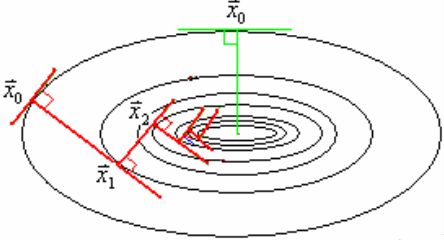
\includegraphics[width=.6\linewidth]{fig/zuisuxiajiangfa.png}
\end{center}

\subsection{Newton法}
\subsubsection{Newton法}

要求有二阶连续偏导数,且Hesse矩阵必须正定且显式。
记$f_k=f(\vec{x}_k),\vec{g}_k=\nabla f(\vec{x}_k),G_k=\nabla^2 f(\vec{x}_k)$。

对Taylor展开式的$f(\vec{x}^*)\approx f(\vec{x}_k)+g(\vec{x}_k)(\vec{x}^*-\vec{x}_k)+\frac{1}{2}(\vec{x}^*-\vec{x}_k)\Transpose G(\vec{x}_k) (\vec{x}^*-\vec{x}_k)$
观察右侧关于$\vec{x}^*$的二次函数,最小值取在$\vec{x}^*-\vec{x}_k = G(\vec{x}_k)^{-1} g(\vec{x}_k)$。
因此选择迭代选择$\vec{x}_{k+1} = \vec{x}_k - G(\vec{x}_k)^{-1}g(\vec{x}_k)$。

对正定二次函数,$G(\vec{x}_k)^{-1} g(\vec{x}_k) = Q^{-1} (Q \vec{x}_k + \vec{b})=\vec{x}_k + Q^{-1}\vec{b}$,
因此下一步直接收敛得到$\vec{x}_{k+1} = -Q^{-1}\vec{b}$。

Newton法的几何解释是使用二次曲面逼近局部,然后取二次曲面上的极小值点为下次的迭代点。

\begin{center}
    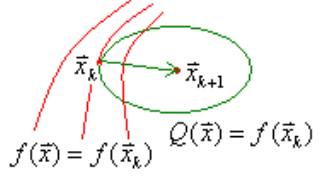
\includegraphics[width=.6\linewidth]{fig/niudunfa.png}
\end{center}

\subsubsection{修正Newton法*}

\subsection{共轭向量法与共轭梯度法}
\subsubsection{共轭向量}
关于从上次迭代点按二阶导数项拟合一个直接指向最小值的方向,得到$\vec{p}_0 Q\vec{p}_1=0$,因此做出以下定义:
\begin{definition}
    若$Q$是$n$阶正定矩阵,非零向量$\VectorComma{\vec{p}}{m}$满足$\vec{p}_i\Transpose Q\vec{p}_j=0$,
    称这组向量是$Q$共轭向量,或者这组向量是$Q$共轭的,这组向量对应的方向称为$Q$共轭方向。
\end{definition}

\begin{theorem}
    $Q$共轭的向量组线性无关。
\end{theorem}

\begin{definition}
    对线性无关向量组$\VectorComma{\vec{p}}{n}$,
    定义全体$\vec{z}=\vec{x}_0+\sum_i a_i\vec{p}_i$构成的集合为
    点$\vec{x}_0$与向量组$\VectorComma{\vec{p}}{n}$生成的线性流形,记为$L[\vec{x}_0;\VectorComma{\vec{p}}{n}]$。
\end{definition}

\subsubsection{共轭方向法}

\begin{theorem}
    给定$n$阶正定矩阵$Q$,$Q$共轭非零向量组$\vec{p}_0,\vec{p}_1,\dots,\vec{p}_{m-1}$,
    任意选取$\vec{x}_0$作为初始点进行$m$次直线搜索得到$\vec{x}_1,\dots,\vec{x}_{m}$,则有:
    $\vec{p}_j\Transpose \nabla f(\vec{x}_m) = 0$,
    且$\vec{x}_m$是二次函数$f(\vec{x})=\frac{1}{2}\vec{x}\Transpose Q \vec{x}+\vec{b}\Transpose\vec{x}+\vec{c}$极小点。
\end{theorem}

因为提供共轭方向的方法不同,共轭方向法有多种。

\subsubsection{共轭梯度法}

共轭梯度法是一种共轭向量法。

\begin{enumerate}
    \item 第一次迭代:
    \begin{enumerate}
        \item 搜索方向取$\vec{p}_0=-\vec{g}_0$;
        \item 步长$t_0=-\frac{\vec{p}_0\Transpose\vec{g}_0}{\vec{p}_0\Transpose Q \vec{p}_0}$;
        \item 迭代点$\vec{x}_1=\vec{x}_0+t_0\vec{p}_0$。
    \end{enumerate}
    \item 第二次迭代:
    \begin{enumerate}
        \item
        搜索方向:考虑和$\vec{p}_0$线性无关,设$\vec{p}_1=\vec{g}_1+\alpha_0 \vec{p}_0$,
        结合共轭条件$\vec{p}_0\Transpose Q \vec{p}_1=0$,
        可得$\alpha_0 = -\frac{\vec{g}_1\Transpose Q \vec{p}_0}{\vec{p}_0\Transpose Q\vec{p}_0}$,
        由此得到$\vec{p}_1$;
        \item 此时步长$t_1 = -\frac{\vec{p}_1\Transpose \vec{g}_1}{\vec{p}_1\Transpose Q \vec{p}_1 }$;
        \item 第二个迭代点$\vec{x}_2=\vec{x}_1+t_1\vec{p}_0$。
    \end{enumerate}
    \item 第$k$次($k>3$):
    \begin{enumerate}
        \item
        搜索方向:考虑和上次的$\vec{p}_{k-1}$线性无关,设$\vec{p}_k=\vec{g}_k+\alpha_{k-1} \vec{p}_{k-1}$,
        结合共轭条件$\vec{p}_k\Transpose Q \vec{p}_{k-1}=0$,
        可得$\alpha_{k-1} = -\frac{\vec{g}_k\Transpose Q \vec{p}_0}{\vec{p}_0\Transpose Q\vec{p}_0}$,
        由此得到$\vec{p}_k$;
        \item 此时步长$t_k = -\frac{\vec{p}_k\Transpose \vec{g}_k}{\vec{p}_k\Transpose Q \vec{p}_k }$;
        \item 第二个迭代点$\vec{x}_k = \vec{x}_{k-1}+t_1\vec{p}_k$。
    \end{enumerate}
\end{enumerate}

\paragraph{不使用Hesse矩阵的共轭梯度法*}

\subsection{拟Newton法}

考虑使用其他矩阵$H$近似Newton法中的$G^{-1}$。
每次使用$\vec{x}_{k+1}=\vec{x}_k - t_k H_k \vec{g}_k$迭代。
然后考查使$H$确实近似$G^{-1}$的条件:
\begin{itemize}
    \item $H_k$正定,以保证每次的搜索方向都是下降方向。
    \item 易于计算的迭代关系,迭代$H_k$的公式称为校正公式。
    \item 逆Newton条件:$\vec{x}_{k+1}-\vec{x}_k\approx H_{k+1} (\vec{g}_{k+1} - \vec{g}_k)$
\end{itemize}

\begin{itemize}
    \item DFP:选择$H_{k+1}=H_k + \alpha_k \vec{u}_k \vec{u}_k\Transpose + \beta_k \vec{v}_k \vec{v}_k\Transpose$
    作为校正公式,其中$\alpha_k,\beta_k,\vec{u}_k,\vec{v}_k$都是待定值。
    \item BFGS(*)
    \item Broyden算法族(*)
\end{itemize}

\subsection{步长加速法*}

\section{约束最优化方法}

最常见的是容许方向法和罚函数法。

\subsection{最优性条件}

\subsubsection{等式约束}
对含有等式约束的最优化问题,
\[
    \begin{array}{ll}
        \min & f(\vec{x})\\
        \SubjectTo & \vec{h}(\vec{x})=0 \\
    \end{array}
\]
令$L=f(\vec{x}) - \sum_i \lambda_i h_i(\vec{x})$,
极值点问题转化为求Lagrange函数的极值点,即
\[
    \nabla L =
    \begin{bmatrix}
        \nabla_{\vec{x}} L \\ \nabla_{\vec{\lambda}} L
    \end{bmatrix} =
    \begin{bmatrix}
        \nabla f(\vec{x}) + \sum\limits_i \lambda_i \nabla h_i(\vec{x}) \\
        h_1(\vec{x}) \\
        \vdots \\
        h_m(\vec{x})
    \end{bmatrix} = \vec{0}
\]
这一方法称为Lagrange乘子法。

\subsubsection{不等式约束的几何最优性条件}
\begin{definition}
    对容许集中一点,去到等号的不等式称为\textkw{起作用约束},否则称为\textkw{不起作用约束}。
    对内点,每个约束都是不起作用约束,对边界点,有至少一个起作用约束。
\end{definition}

\begin{definition}
    对从一点$\vec{x}$和方向向量$\vec{p}$,
    若$\exists \delta>0$使得$\forall t\in (0,\delta),\vec{x}+t\vec{p}\in D$,
    称为\textkw{容许方向}。
\end{definition}

\begin{definition}[锥。凸锥。]
\end{definition}

\begin{definition}
    全体容许方向向量构成\textkw{容许方向锥}。
    全体下降方向向量构成\textkw{下降方向锥}。
\end{definition}

\begin{theorem}[几何最优性条件]
    下降方向锥与容许方向锥交集为空。
\end{theorem}
这是一个必要条件。

\subsubsection{F-J条件}
\begin{lemma}[Farkas引理]
    对$n$维向量$\VectorComma{a}{m},b$,有:
    $a_i\Transpose p>0,i=1,2,\dots,m\Rightarrow b\Transpose p>0\Leftrightarrow \exists \VectorComma{\gamma}{m}>0,b=\sum\limits_i \gamma_i a_i$。
\end{lemma}

\begin{lemma}[Gordan引理]
    对$n$维向量$\VectorComma{a}{m}$,有:
    $\nexists p,\vec{a}\Transpose p<0,i=1,2,\dots,m \Rightarrow \exists \VectorComma{\gamma}{m}\geq 0,b=\sum\limits_i \gamma_i a_i=\vec{0}$。
\end{lemma}

\begin{theorem}[Fritz-John条件]
    $\vec{x}^*$是极小点$\Rightarrow\exists \mu_0,\linebreak[1]\mu_1,\linebreak[1]\dots,\linebreak[1]\mu_m\text{不全为零}$,使得:
    \[
        \begin{cases}
            \mu_0\nabla f(\vec{x}^*) - \sum\limits_i\mu_i\nabla s_i(\vec{x}^*) = 0 &\quad\text{(Lagrange函数)} \\
            \mu_i s_i(\vec{x}^*) = 0, i=1,2,\dots,m & \quad\text{(互补松弛条件)} \\
            \mu_i \geq 0, i=1,2,\dots,m & \\
        \end{cases}
    \]
    这个必要条件称为F-J条件,满足F-J条件的所有点称为F-J点。
    式中的$\mu_0,\mu_1,\dots,\mu_m$称为Lagrange乘子。
\end{theorem}

\subsubsection{K-T条件}
约束F-J条件的$\mu_0=1$得到K-T条件。
\begin{theorem}[Kuhn-Tucker条件]
    $\vec{x}^*$是极小点$\Rightarrow\exists \mu_1,\linebreak[1]\dots,\linebreak[1]\mu_m$,使得:
    \[
        \begin{cases}
            \mu_0\nabla f(\vec{x}^*) = \sum\limits_i\mu_i\nabla s_i(\vec{x}^*) &\quad\text{(Lagrange函数)} \\
            \mu_i s_i(\vec{x}^*) = 0, i=1,2,\dots,m & \quad\text{(互补松弛条件)} \\
            \mu_i \geq 0, i=1,2,\dots,m & \\
        \end{cases}
    \]
    这个必要条件称为K-T条件或KKT条件(KKT指Karush-Kuhn-Tucker),满足K-T条件的所有点称为K-T点。
\end{theorem}

\begin{theorem}
    起作用的$\nabla s$线性无关,且$\mu_0\neq 0$的F-J点必为K-T点。
\end{theorem}

\begin{theorem}
    对凸规划,其中$f$可微凸函数,$s$可微凹函数,$h$线性函数,则K-T点都是全局最优点。
\end{theorem}

\subsection{外部罚函数法}
对最优化问题,定义增广目标函数
\[
    \begin{split}
        F(\vec{x},\mu) &= f(\vec{x}) + \mu \alpha(\vec{x}) \\
        \alpha(\vec{x}) &= \sum_j [h_j (\vec{x})]^2 + \sum_i [s_i(\vec{x})]^2 u(s_i(\vec{x})) \\
    \end{split}
\]
$F$称为增广目标函数,
$\mu$为罚因子,第二项$\mu\alpha(\vec{x})$称为惩罚项,
其中的$u(t)$是一个阶跃函数,定义为
\[
    u(t)=\begin{cases}0,t \geq 0\\1,t<0\end{cases}
\]

\begin{theorem}
    给定$\mu$,若$\vec{x}_\mu$是无约束问题$\min F(\vec{x},\mu)$的极小点,
    则$\vec{x}_\mu$是有约束问题$\min f(\vec{x}) \SubjectTo h_j(\vec{x})=0, s_i(\vec{x})\geq 0$的极小点的
    充要条件是$\vec{x}_\mu$是有约束问题的容许点。
\end{theorem}

对于一般的$\vec{x}\notin C$,需要增大$\mu$计算,
一般认为$\mu=1,2,\dots$得到序列$\{\vec{x}_k\}$,
则若$\{\vec{x}_k\}$收敛,一定能收敛在极小点。
这种方法称为\textkw{外部罚函数法}或\textkw{外点法}。
这种通过解无约束问题进而解决有约束问题的方法,也称为``序列无约束最小化技术''(SUMT)。

\subsection{内部罚函数法}
外点法取在外部并逐渐向容许集边界移动,因此其可能难以取到容许集内的点,
或者可能函数在容许集外根本无法定义,导致不能用外点法计算出极小点。
为保证迭代点总是内点,则产生了内部罚函数法。

初始点$\vec{x}_0$选择内点,然后设计障碍函数
\[
    \begin{split}
        F(\vec{x},\mu) &= f(\vec{x}) + \mu\beta(\vec{x}) \\
        \beta(\vec{x}) &= \sum_i \frac{1}{s_i(\vec{x})} \\
    \end{split}
\]
$F$为障碍函数,
$\mu$为罚因子,第二项$\mu\beta(\vec{x})$为惩罚项。
$\beta$也可以取如$\sum\ln \frac{1}{s(\vec{x})}, \sum \frac{1}{s^2(\vec{x})}, \sum\frac{1}{s(\vec{x}) u[-s(\vec{x})]}$等的函数。

选择一个内点作为初始点,通过$\mu\to 0^+$,得到极小点。

注意内部罚函数法有无法处理等式约束的严重缺陷,
产生的结合两种罚函数法的优势得到了混合罚函数法。

\subsection{乘子法}
外部罚函数法中,随着罚因子增大,Hesse矩阵条件数增大,数值计算的稳定性变差导致计算结果不精确,
于是产生了乘子法。

\paragraph{H乘子法*}
\paragraph{R乘子法*}

\subsection{Zoutendijk容许方向法*}

\section{多目标规划}
同时对多个目标进行优化即多目标规划问题。

\subsection{数学模型}
不等式约束转换为大于等于后,可得数学模型:
\[
    \begin{array}{ll}
        \min & f_1(\VectorComma{x}{n}) \\
        \min & f_2(\VectorComma{x}{n}) \\
        & \dots \\
        \min & f_p(\VectorComma{x}{n}) \\
        \max & g_1(\VectorComma{x}{n}) \\
        \max & g_2(\VectorComma{x}{n}) \\
        & \dots \\
        \max & g_q(\VectorComma{x}{n}) \\
        \SubjectTo & s_i(\VectorComma{x}{n})\geq 0 \\
        & h_j(\VectorComma{x}{n}) = 0 \\
    \end{array}
\]
将最大转换为最小,写成向量形式,记
\[
    \begin{split}
        \vec{x} &= (\VectorComma{x}{n})\Transpose \\
        \vec{f}(\vec{x}) & =(f_1(\vec{x}),f_2(\vec{x}),\dots,f_p(\vec{x}),f_{p+1}(\vec{x}),\dots,f_r(\vec{x}))\Transpose \\
        f_{p+k}(\vec{x}) & = -g_{k}(\vec{x}) \\
        D &= \{\vec{x}\mid s_i(\vec{x})\geq 0,h_i(\vec{x}) = \vec{0}\} \\
    \end{split}
\]
则原问题可记为
\[
    \mathbf{v-}\min_{\vec{x}\in D} \vec{f}(\vec{x})
\]
称为向量极小化模型,$\vec{f}(\vec{x})$称为向量目标函数,其分量称为分量目标函数。

对各分量目标函数为线性的情况,可通过线性替换使得$\vec{s}(\vec{x})$转化为
\[
    \begin{array}{rl}
        \mathbf{v-}\min\limits_{\vec{x}} & \vec{f}(\vec{x}) = C\vec{x} \\
        \SubjectTo & A\vec{x} = \vec{b} \\
        & \vec{x} \geq \vec{0} \\
    \end{array}
\]

\subsection{解的概念与性质}
\begin{definition}[向量的序关系]
    \begin{gather*}
        \vec{a} < \vec{b} \Leftrightarrow \vec{b} > \vec{a} \Leftrightarrow \forall i,a_i<b_i \\
        \vec{a} \leq \vec{b} \Leftrightarrow \vec{b} \geq \vec{a} \Leftrightarrow \forall i,a_i\leq b_i \\
        \vec{a} \prec \vec{b} \Leftrightarrow \vec{b} \succ \vec{a} \Leftrightarrow \forall i, a_i\leq b_i \land \exists i, a_i\neq b_i\\
    \end{gather*}
\end{definition}

\begin{definition}[不同程度的最优解]
    为确定``好''解,定义:
    \begin{itemize}
        \item
        对$\vec{f}(\vec{x})$,给定$\vec{x}^*$,
        若$\forall \vec{x} \in D, \vec{f}(\vec{x}) \geq \vec{f}(\vec{x}^*)$,
        则称$\vec{x}^*$为\textkw{绝对最优解}。
        全体绝对最优解的集合为\textkw{绝对最优解集},记作$X^*(\vec{f},D)$。
        \item
        对$\vec{f}(\vec{x})$,给定$\vec{x}^*$,
        若$\nexists \vec{x} \in D, \vec{f}(\vec{x}) \prec \vec{f}(\vec{x}^*)$,
        则称$\vec{x}^*$为\textkw{有效解}或\textkw{Pareto解}。
        全体有效解的集合为\textkw{有效解集},记作$P(\vec{f},D)$。
        \item
        对$\vec{f}(\vec{x})$,给定$\vec{x}^*$,
        若$\nexists \vec{x} \in D, \vec{f}(\vec{x}) < \vec{f}(\vec{x}^*)$,
        则称$\vec{x}^*$为\textkw{弱有效解}。
        全体弱有效解的集合为\textkw{弱有效解集},记作$P_w(\vec{f},D)$。
    \end{itemize}
\end{definition}

\begin{theorem}
    $X^* \subseteq P \subseteq P_w \subseteq D$,
    且$X^*=\bigcap\limits_i X^*_i,\bigcup\limits_i X^*_i\subseteq P_w$。
    其中$X^*,P,P_w$分别为绝对最优、有效、弱有效解,
    $X^*_i$为第$i$个分量目标函数的最优解集。
\end{theorem}

\begin{theorem}
    若$X^*\neq \emptyset$,则$P=X^*$。
    若$D$是凸集,每个分量目标函数$f_i$是凸函数,则$P=P_w$。
\end{theorem}

\subsection{评价函数法}
\begin{definition}[多元函数单调性]
    多元函数$\varphi:\mathbb{R}^r\to\mathbb{R}$:
    若$\forall \vec{z}_1<\vec{z}_2,\varphi(\vec{z}_1)<\varphi(\vec{z}_2)$,称$\varphi(\vec{z})$单调增函数;
    若$\forall \vec{z}_1\prec\vec{z}_2,\varphi(\vec{z}_1)<\varphi(\vec{z}_2)$,称$\varphi(\vec{z})$严格单调增函数。
\end{definition}

\begin{theorem}
    对多目标规划$\vec{f}(\vec{x})$,
    考虑$\min\limits_{x\in D} \varphi(\vec{f}(\vec{x}))$有极小点$\vec{x}^*$,则:
    \begin{itemize}
        \item 若$\varphi$是严格增函数,$x^*\in P(\vec{f}, D)$
        \item 若$\varphi$是增函数,$x^* \in P_w(\vec{f}, D)$
    \end{itemize}
\end{theorem}
称这样的$\varphi$为评价函数。

\subsubsection{常见评价函数}

\paragraph{线性加权和}
取评价函数$\varphi(\vec{z})=\vec{u}\vec{z},u_i\geq 0,\sum u_i=1$为\textkw{线性加权和函数},
其中$\vec{u}$为\textkw{权向量},且:
$\vec{u}>0$时,严格单调增;$\vec{u}\succ \vec{0}$时,单调增。
这样的方法称为\textkw{线性加权和法}。

\paragraph{理想点函数}
取评价函数$\varphi(\vec{z})=\|\vec{z}-\vec{z}^*\|$为\textkw{理想点函数},
其中$\vec{z}^*$是每个分量函数能取到的最小值,称为\textkw{理想点},
这样的方法称为\textkw{理想点法}。

\paragraph{平方加权函数}
考虑理想点函数中范数进行平方,取加权的二次方和的情况,
取评价函数$\varphi(\vec{z})=\sum\limits_i (\vec{z}_i-\vec{z}_i^*)$。
这样的方法称为\textkw{平方加权和法}。

\paragraph{极大函数}
取评价函数$\varphi(\vec{z})=\max\{z_i\}$或加权的$\max\{u_i z_i\}$,
这样的方法称为\textkw{极大极小法}。
由于直接求这个极大值的极小值较难,通常转化为$\min v \SubjectTo u_i f_i(\vec{x})\leq v,x\in D$来求解,
其中$v$称为松弛变量。

\subsubsection{权重的确定}
\paragraph{去量纲处理}
首先需要将各不同目标函数的量纲去除。

\paragraph{老手法}
选择多位相关专家和有实践经验的工作者,统计其对不同项目的权重的估计值,然后求取平均。
求平均后需要检查每个人与平均结果的最大偏差,若偏差足够小则认为大家的经验无差别,可以使用,
否则需要再次进行协商调整并重复此流程。

\paragraph{$\alpha$法}
借助各分量目标函数在容许集上的极小值点确定权重的方法。
通过最小化不同的分量目标函数得到极小值点$\VectorComma{\vec{x}^*}{r}$,
在自变量取这些值时得到向量目标函数的取值$\vec{z}^*_i=\vec{f}(\vec{x}^*_i)$。
若这是$r$个不同的点,撑起一个$r$维空间中的超平面,
设$\vec{u}\Transpose \vec{z}=\alpha$,
改变合适的$\alpha$值使得$\vec{u}$每个分量非负且和为$1$,
则得到一个可用的权重向量$\vec{u}$。

\section{标量的矩阵求导术}
\begin{definition}
    对矩阵函数$f:F^{m\times n}\to F$,定义对矩阵的导数
    $\frac{\partial f}{\partial A}=\left(\frac{\partial f}{\partial a_{ij}}\right)_{m\times n}$
\end{definition}

\begin{itemize}
    \item $f(A)=X\Transpose AY,\frac{\partial f}{\partial A}=XY\Transpose$
    \item $f(A)=\TraceOf(AB)=\TraceOf(BA),\frac{\partial f}{\partial A} = B\Transpose$
    \item $f(A)=\TraceOf(A\Transpose C)=\TraceOf(CA\Transpose)=A\bullet C,\frac{\partial f}{\partial A}=C$
    \item $f(A)=\TraceOf(A\Transpose A)=\TraceOf(AA\Transpose)=\|A\|_F^2,\frac{\partial f}{\partial A}=2A$
    \item $f(A)=\TraceOf(A\Transpose AB),\frac{\partial f}{\partial A}=AB+AB\Transpose$
    \item $f(A)=\TraceOf(A\Transpose BA),\frac{\partial f}{\partial A}=BA+B\Transpose A$
    \item $f(A)=\TraceOf(PAQ)=\TraceOf(AQP),\frac{\partial f}{\partial A}=P\Transpose Q\Transpose$
\end{itemize}
